\documentclass{ximera}

\author{Anna Davis} \title{MTH 160 Homework 4} 

\begin{document}

\begin{abstract}

\end{abstract}
\maketitle
 \textit{Certificate due: 2/10/2021 at 11:59 p.m.}

\section{Lecture 7}
\begin{problem}\label{prob:160hom3prob3}
The graph of a function and its inverse are shown below.  
\begin{image}
   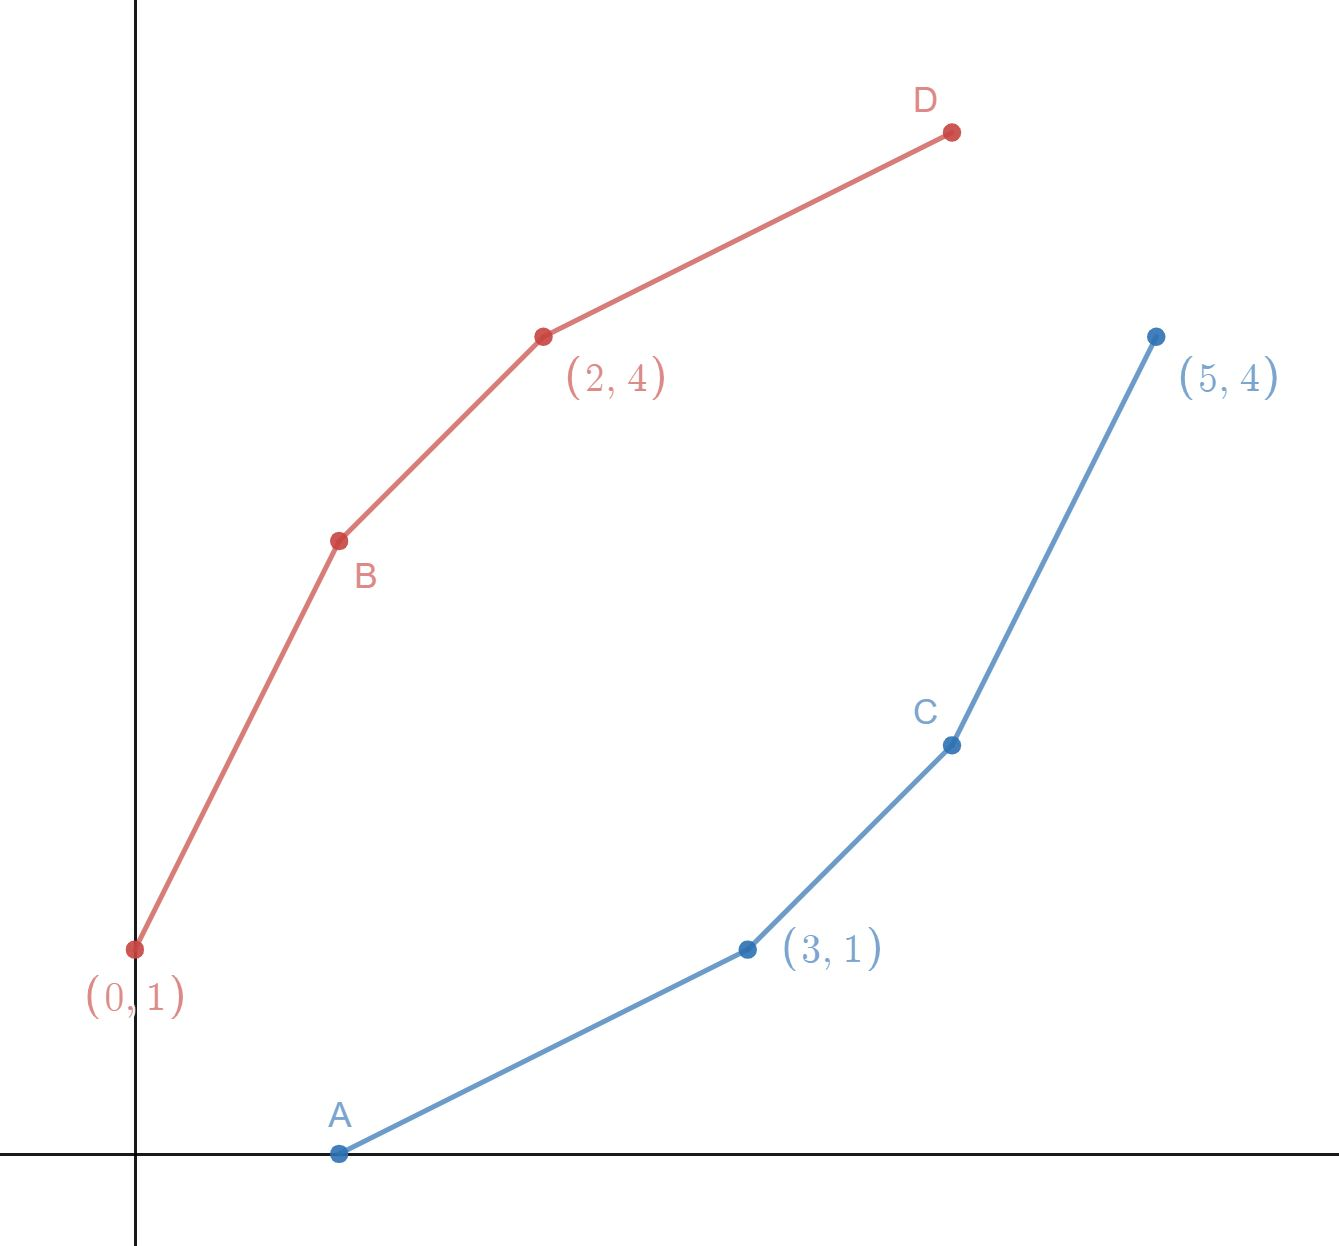
\includegraphics[height=1in]{160H3pic1.jpg}
 \end{image}
Find the coordinates of $A, B, C, D$.
$$A=(\answer{1},\answer{0}),\quad B=(\answer{1},\answer{3}),\quad C=(\answer{4},\answer{2}),\quad D=(\answer{4},\answer{5})$$
The two graphs are symmetric about the line
$y=\answer{x}$.
\end{problem}
\begin{problem}\label{prob:160hom3prob4}
Find $f^{-1}$.
\begin{enumerate}
    \item $f(x)=5x+7$
    $$f^{-1}(x)=\answer{\frac{1}{5}}x-\answer{\frac{7}{5}}$$
    \item $f(x)=\frac{1}{x+10}$
    $$f^{-1}(x)=\answer{\frac{1}{x}-10}$$
\end{enumerate}

\end{problem}



 \section{Lecture 8}
\begin{problem}\label{prob:160hom4prob1} 
 Find the slope for each pair of points.  Enter exact number.
 \begin{enumerate}
     \item $(3, -10)$ and $(-10,4)$.
     $$m=\answer{-\frac{14}{13}}$$
     \item $(-2, -1)$ and $(-4,-7)$.
     $$m=\answer{3}$$
     \item $(5, -4)$ and $(12,-4)$.
     $$m=\answer{0}$$
 \end{enumerate}
 \end{problem}
 
 \begin{problem}\label{prob:160hom4prob2} 
 Each line below is labeled with a letter.  Arrange the letters in an increasing order by slope.  Enter your response as a single string of capital letters (e.g. ABCDEF) - no spaces, no commas, all caps.
 
 \begin{image}
   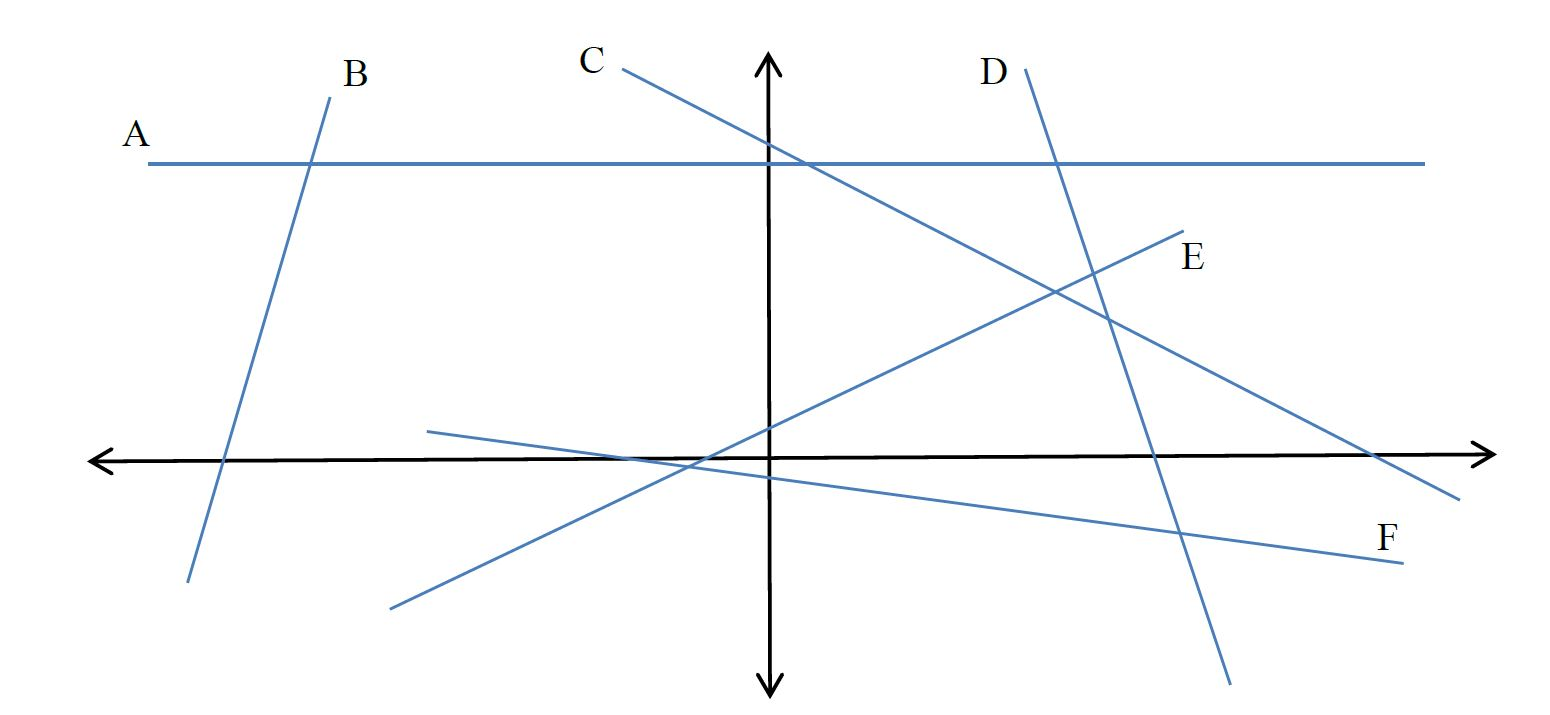
\includegraphics[height=1in]{160H4pic1.jpg}
 \end{image}
 $$\answer[format=string]{DCFAEB}$$
 \end{problem}
 \section{Lecture 9}
\begin{problem}\label{prob:160hom4prob3}
Find an equation, in slope-intercept form, of each line described below.
  \begin{enumerate}
      \item Line passing through $(-1, 7)$ and $(-3, 15)$.
      $$y=\answer{-4x+3}$$
      \item Line passing through $(2, -3)$ and $(-2, -1)$.
      $$y=\answer{-\frac{1}{2}x-2}$$
      \item Line passing through $(1,2)$ and is parallel to $y=10x-10$.
      $$y=\answer{10x-8}$$
      \item Line passing through $(6, -5)$ and is perpendicular to $y=-3x+1$.
      $$y=\answer{\frac{1}{3}x-7}$$
  \end{enumerate}
\end{problem}

\begin{problem}\label{prob:160hom4prob4}
Find the equation of each line whose graph is given below.

\begin{image}
   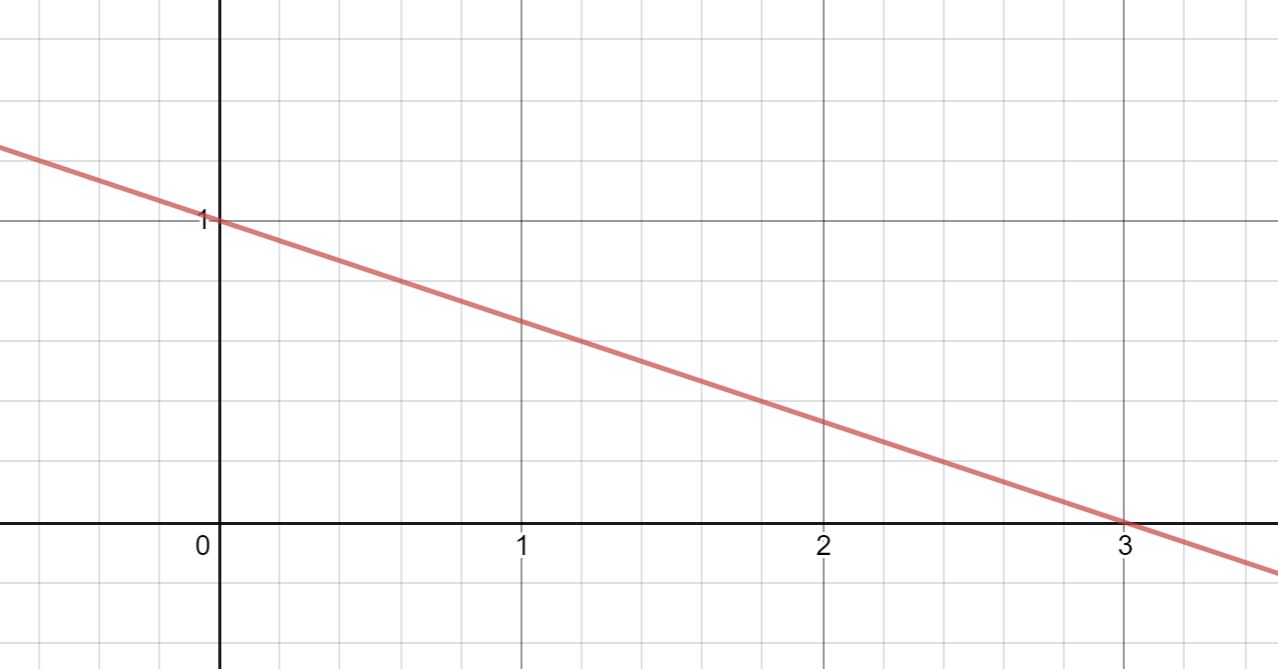
\includegraphics[height=1in]{160H4pic2.jpg}
 \end{image}
 
 $$y=\answer{-\frac{1}{3}x+1}$$
 
 \begin{image}
   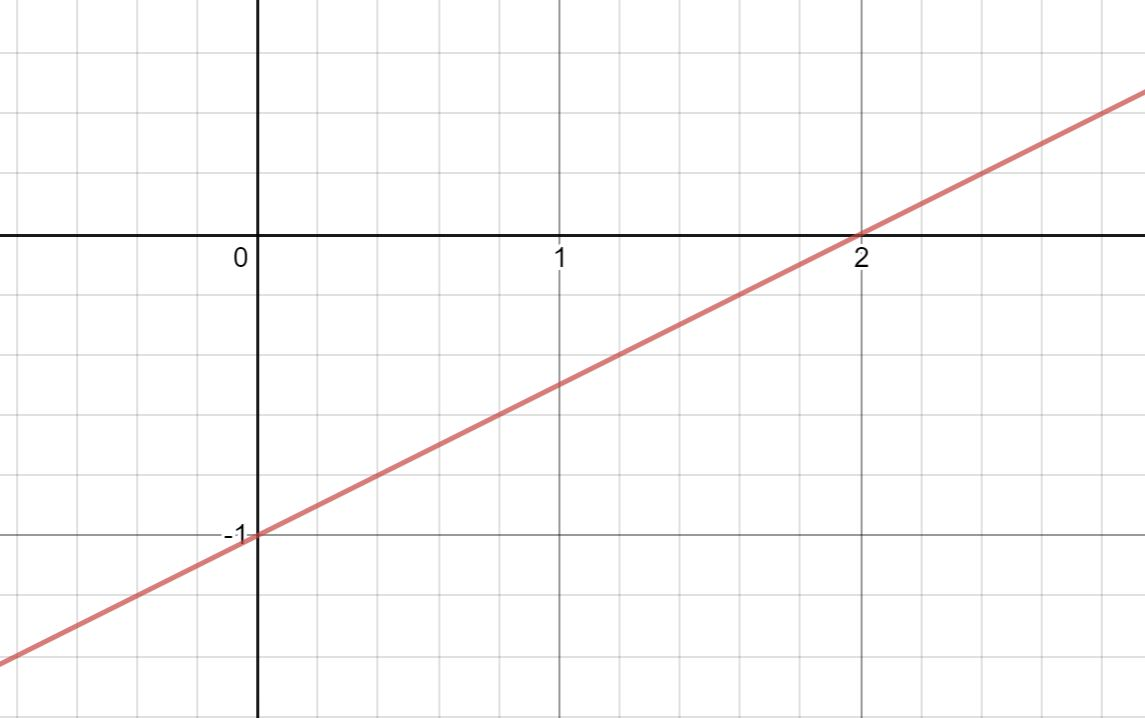
\includegraphics[height=1in]{160H4pic3.jpg}
 \end{image}
 
 $$y=\answer{\frac{1}{2}x-1}$$

\end{problem}

\begin{problem}\label{prob:160hom4prob5}
Find the $x$ and $y$ intercepts for a line whose graph is given below.

 
 \begin{image}
   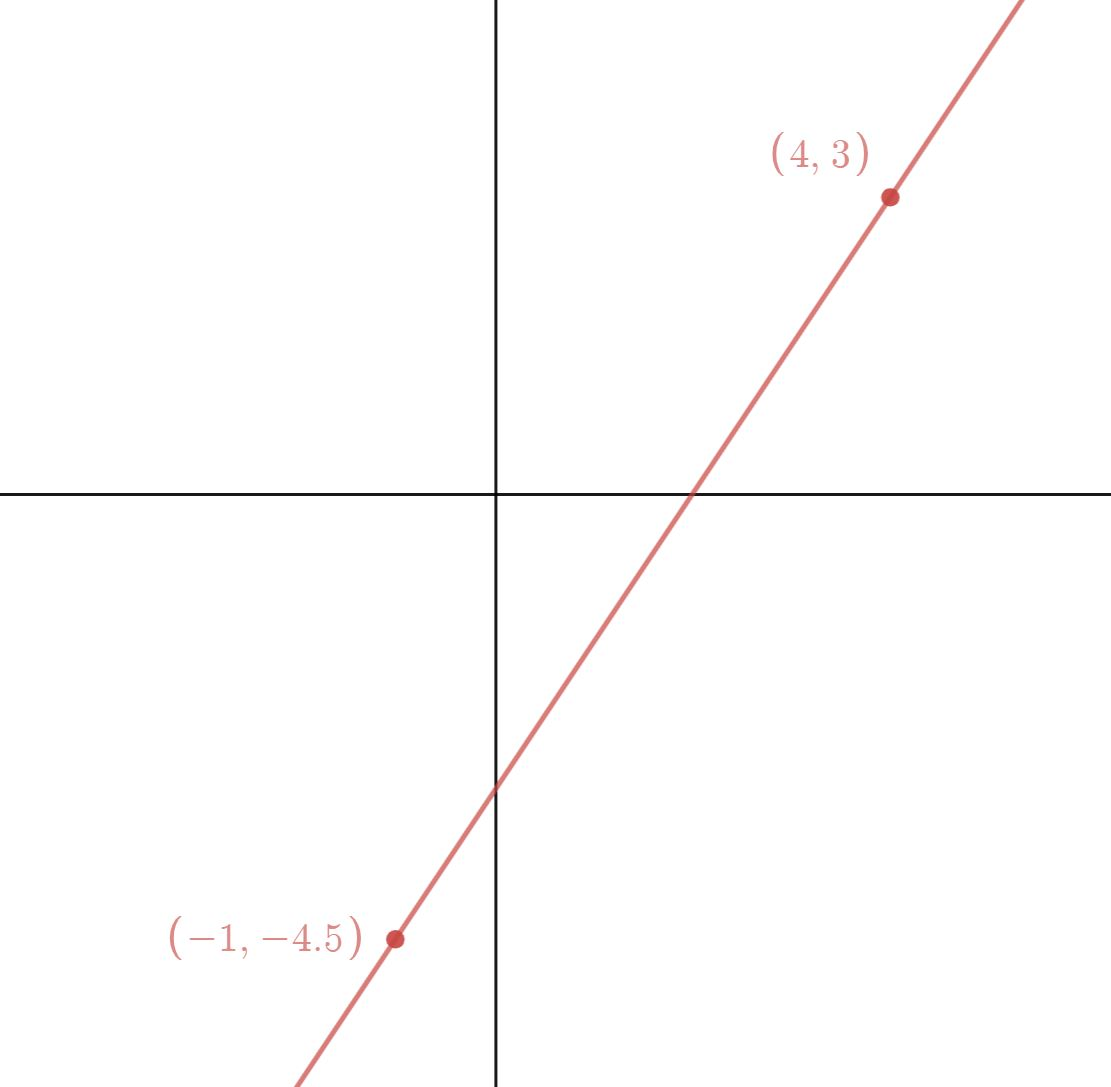
\includegraphics[height=1in]{160H4pic4.jpg}
 \end{image}
 
 $$x\mbox{-intercept}: (\answer{2},0),\quad y\mbox{-intercept}: (0, \answer{-3})$$
\end{problem}

\begin{problem}\label{prob:160hom4prob6}
Find the equation of the blue line if it is known that the the blue line is (a) parallel to the red line (Figure 1); (b) perpendicular to the red line (Figure 2).
\begin{image}
   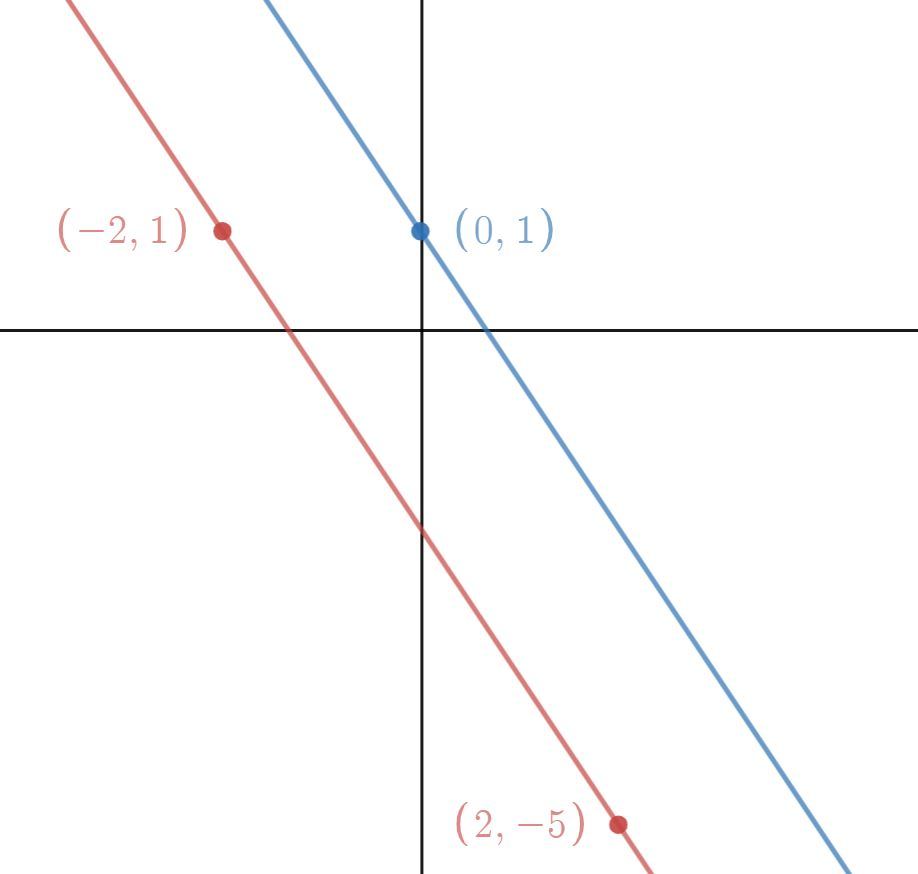
\includegraphics[height=1in]{160H4pic5.jpg}
 \end{image}
 \begin{center}
     Figure 1
 \end{center}
 Equation of the blue line: $y=\answer{-1.5x+1}$
 \begin{image}
   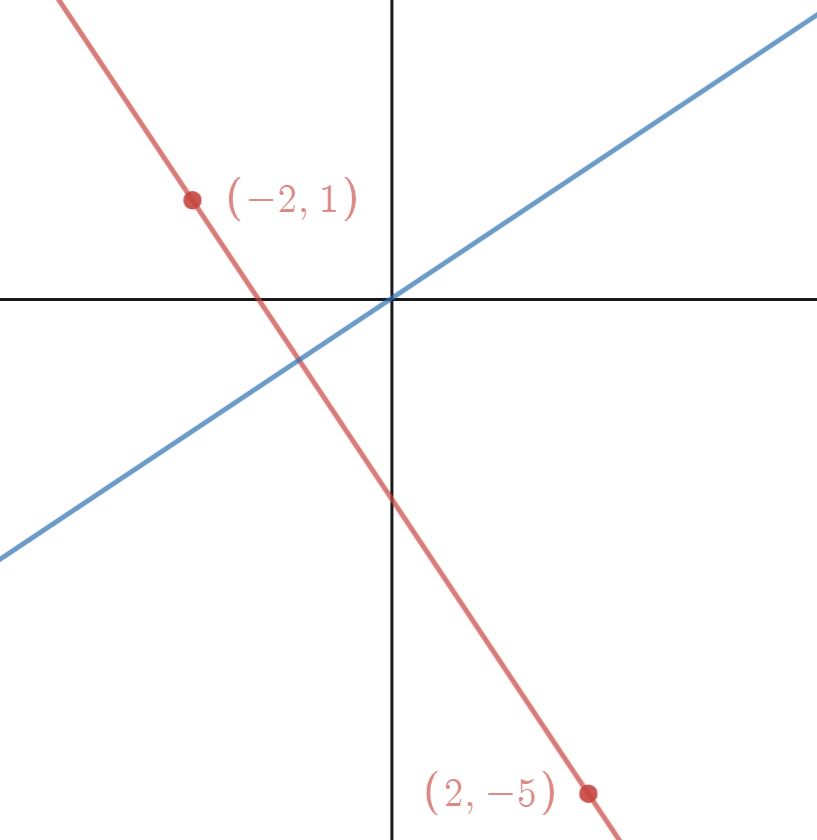
\includegraphics[height=1in]{160H4pic6.jpg}
 \end{image}
 \begin{center}
     Figure 2
 \end{center}
  Equation of the blue line: $y=\answer{\frac{2}{3}x}$
\end{problem}
\end{document}